\subsection{Overview}
Version 1 was another version that we did not use as the final interface for data collection. However, a few major changes in 
For version 1 onward, we decided to host our website on Amazon Mechanical Turk (AMT), which is a crowd-sourcing website that hosts different annotation tasks to collect datasets for machine learning. From this point onward, we will use the word \textit{turker} to refer to annotators that we recruit on AMT. We have to design the following sections for the task: 
\begin{itemize}
    \item the main task to collect data
    \item instructions and requirements to describe the tasks and specify what the annotation should include and what it should not include
    \item a qualification task accompanying the main task to train the turkers to produce high-quality annotations
\end{itemize}
After deployment, we realized that a few major problems from this design: (1) due to the subjective nature of drawing, it was hard to understand in what ways some annotators are illustrating the given prompts, thus making it difficult to determine the quality of the annotations; (2) turkers are taking more than 30 minutes for each task, showing that providing both sketches and descriptions are inefficient; (3) some turkers are unable to provide descriptions that align with the objects they meant to annotate for; for example, in one step, they drew both eyes and hair, but they only annotate ``big eyes''.      

\subsection{Interface Design}

\subsubsection{Main Task}
Compare to version 0, we make the following changes to the task interface: 
\begin{enumerate}
    \item Since turkers are paid based on time spent on the task, we decided to forsake the functionality related to the recording and replaying the drawing board.
    \item Since we decide to not limit the drawings to be compositions of basic geometric objects, we removed the step to select primitive shape preceding drawing each component.
\end{enumerate}

\begin{figure*}[!htb]
\begin{subfigure}{\textwidth}
    \centering
    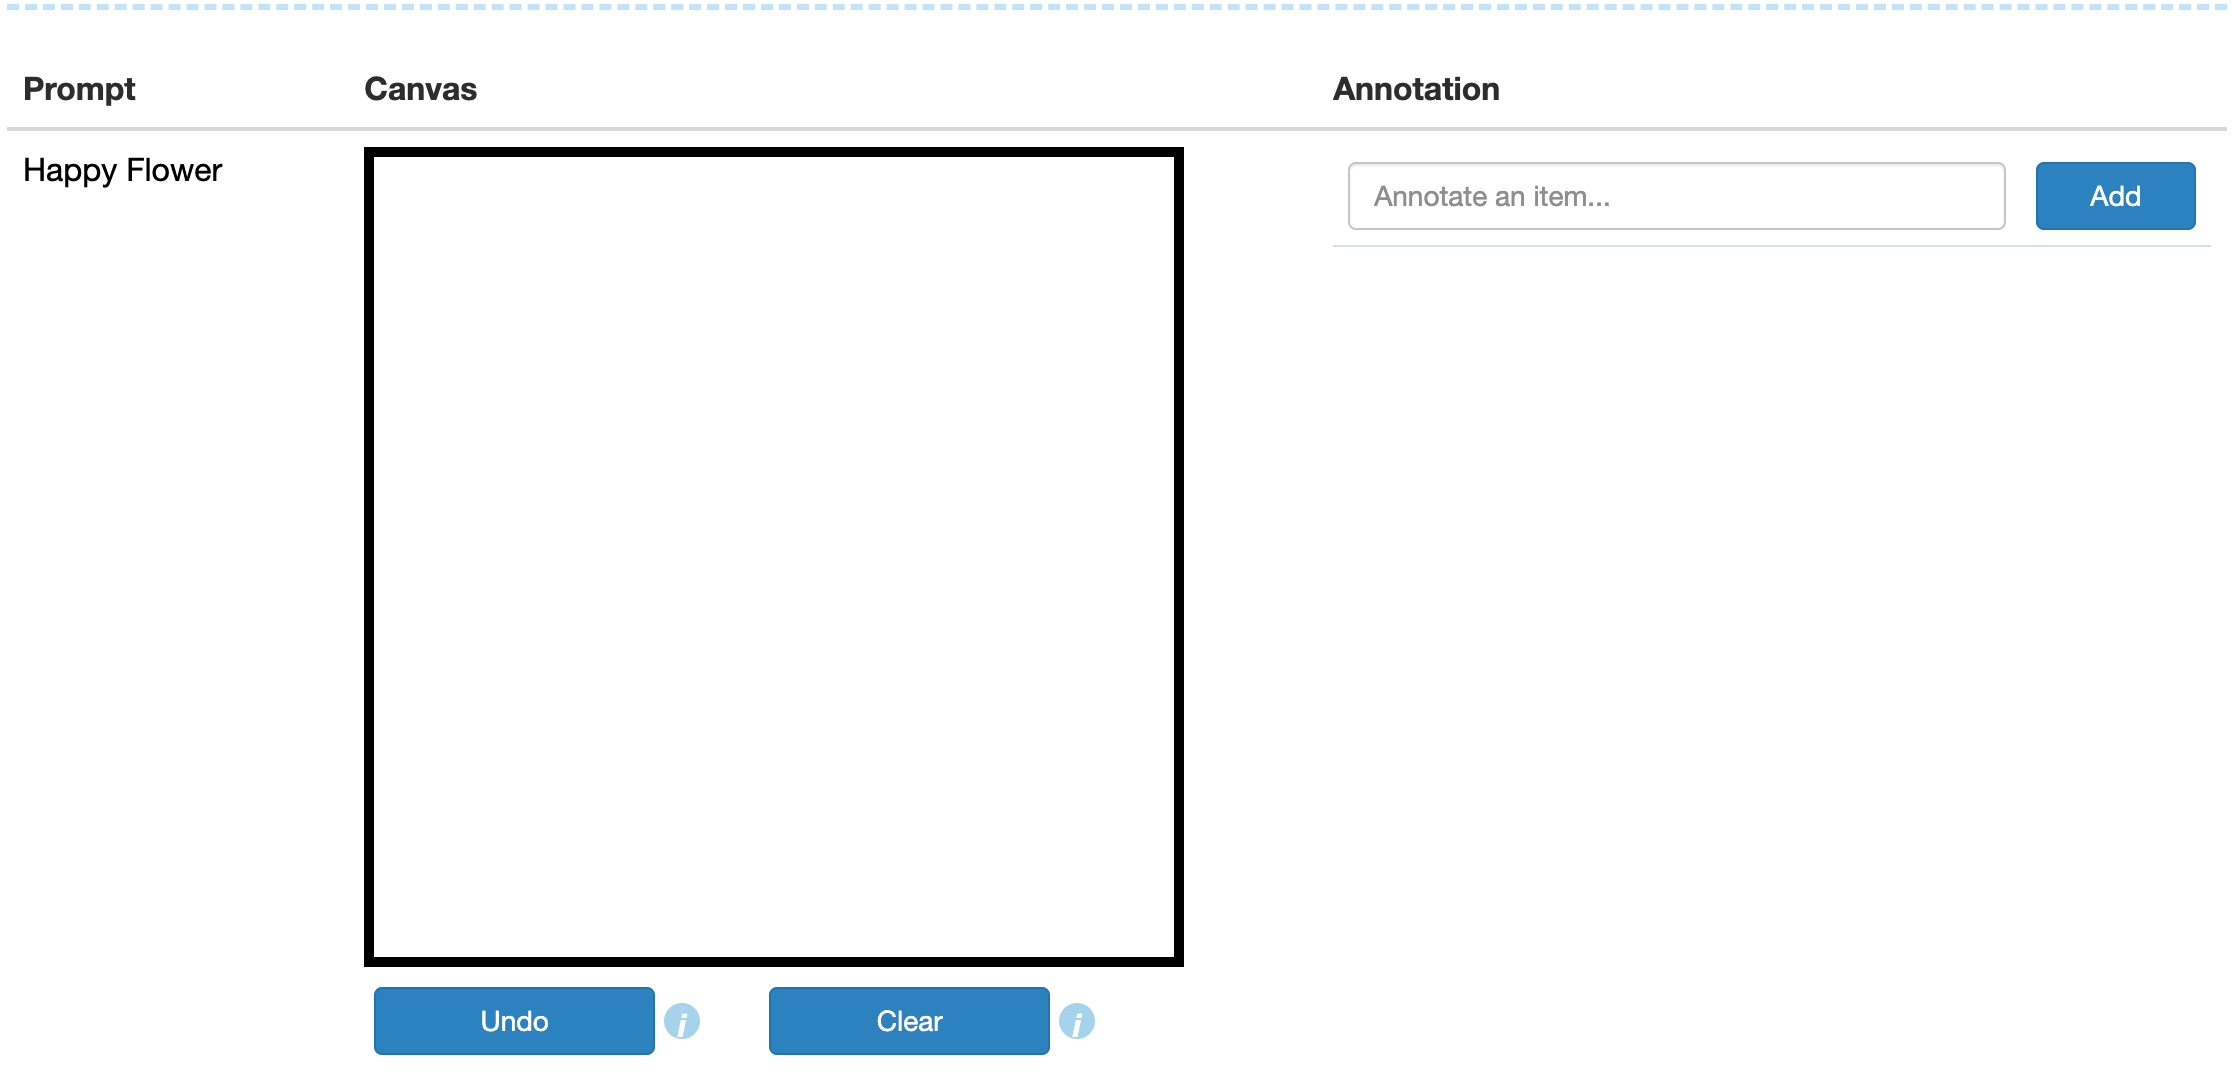
\includegraphics[width=.8\linewidth]{data_collection/v1_empty_table.png}  
    \caption{Main task interface at the start of annotation.}
    \label{v1.main_task.1.a}
\end{subfigure}
\newline
\begin{subfigure}{\textwidth}
    \centering
    % include third image
    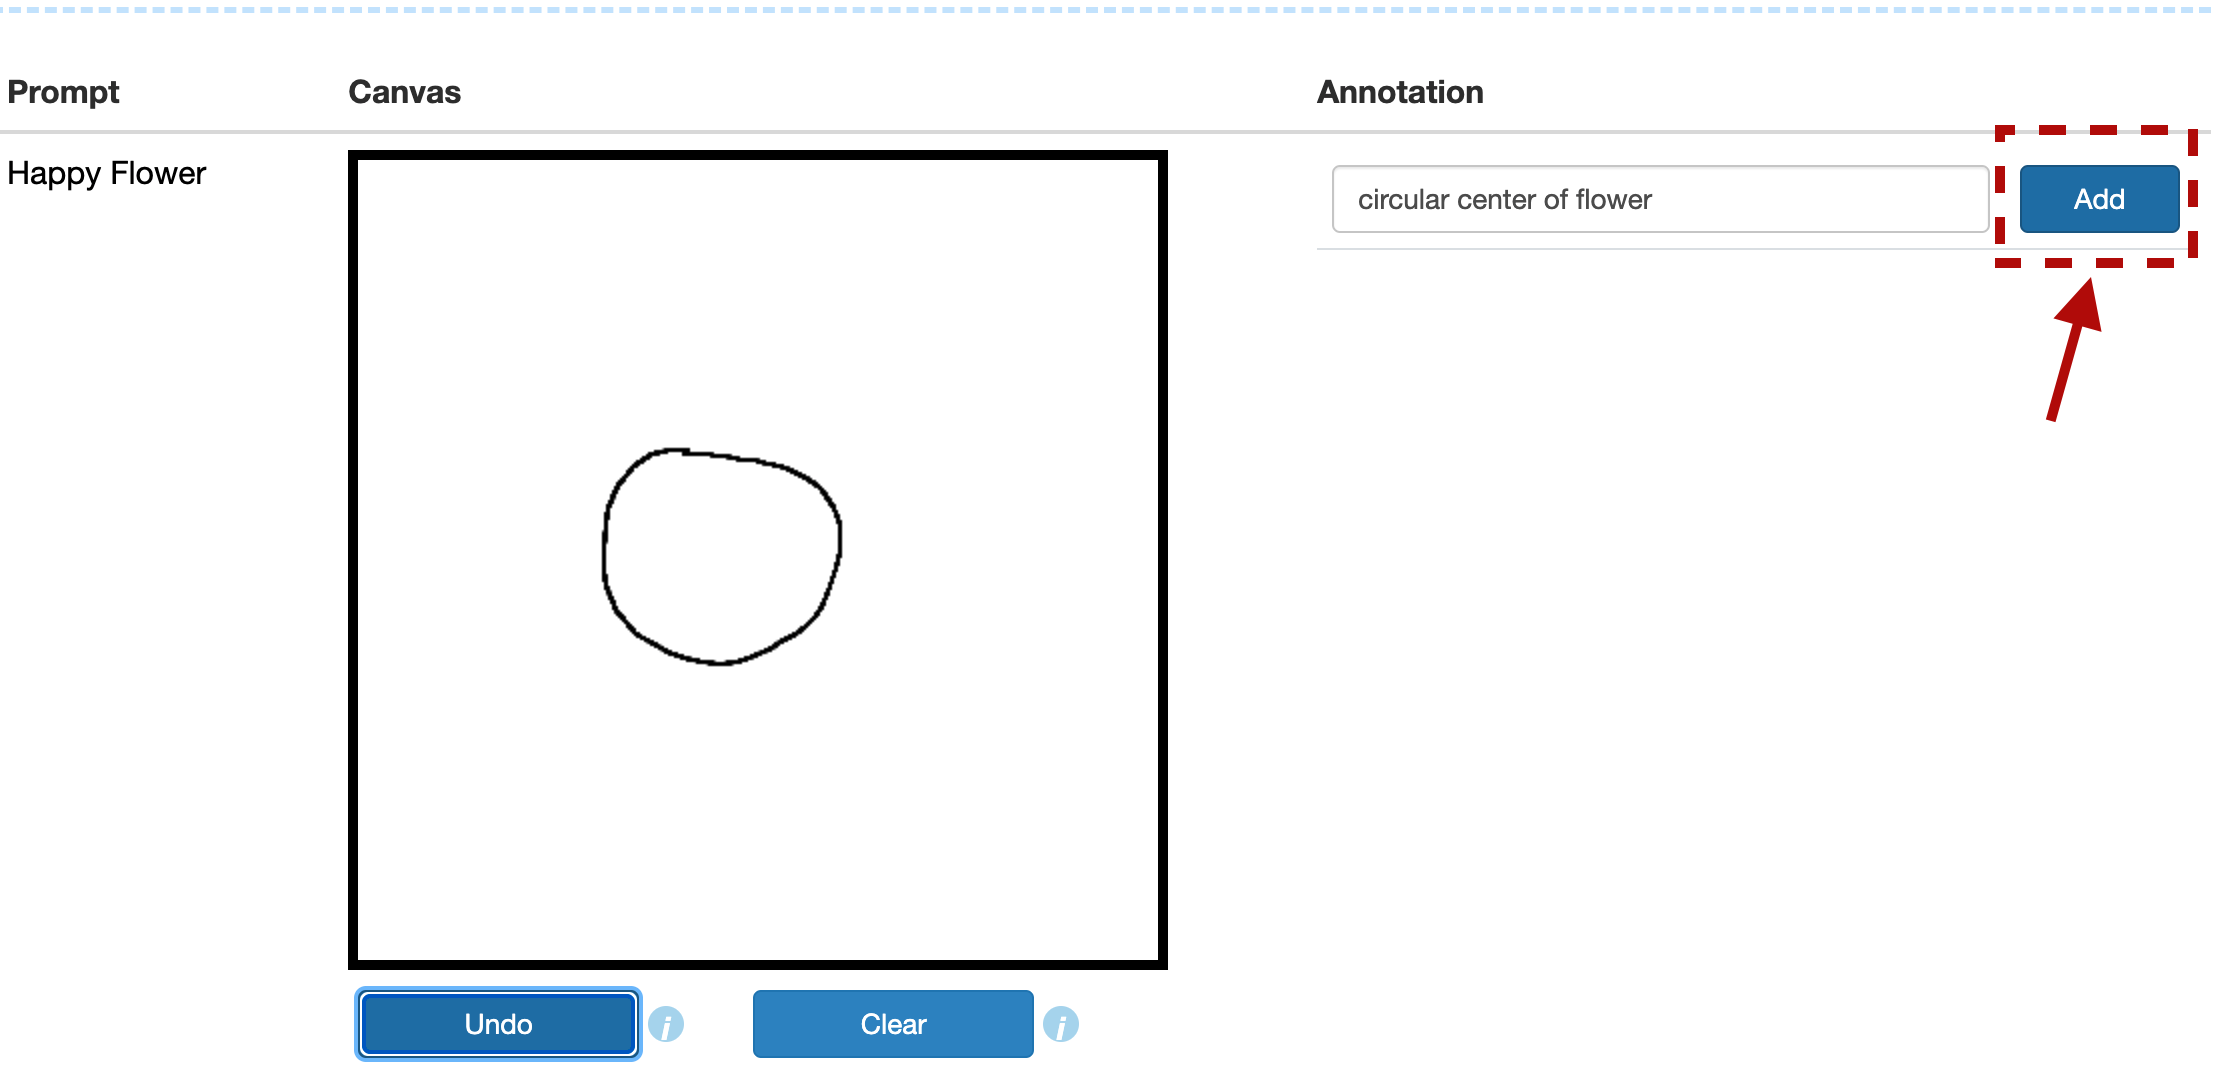
\includegraphics[width=.8\linewidth]{data_collection/v1_before_enter_text.png}  
    \caption{Main task interface before adding textual descriptions for the drawing in the given step. Red arrow and box shows where to click to add the text.}
    \label{v1.main_task.1.b}
\end{subfigure}
\end{figure*}

\begin{figure*}[!htb]
\ContinuedFloat
\begin{subfigure}{\textwidth}
    \centering
    % include third image
    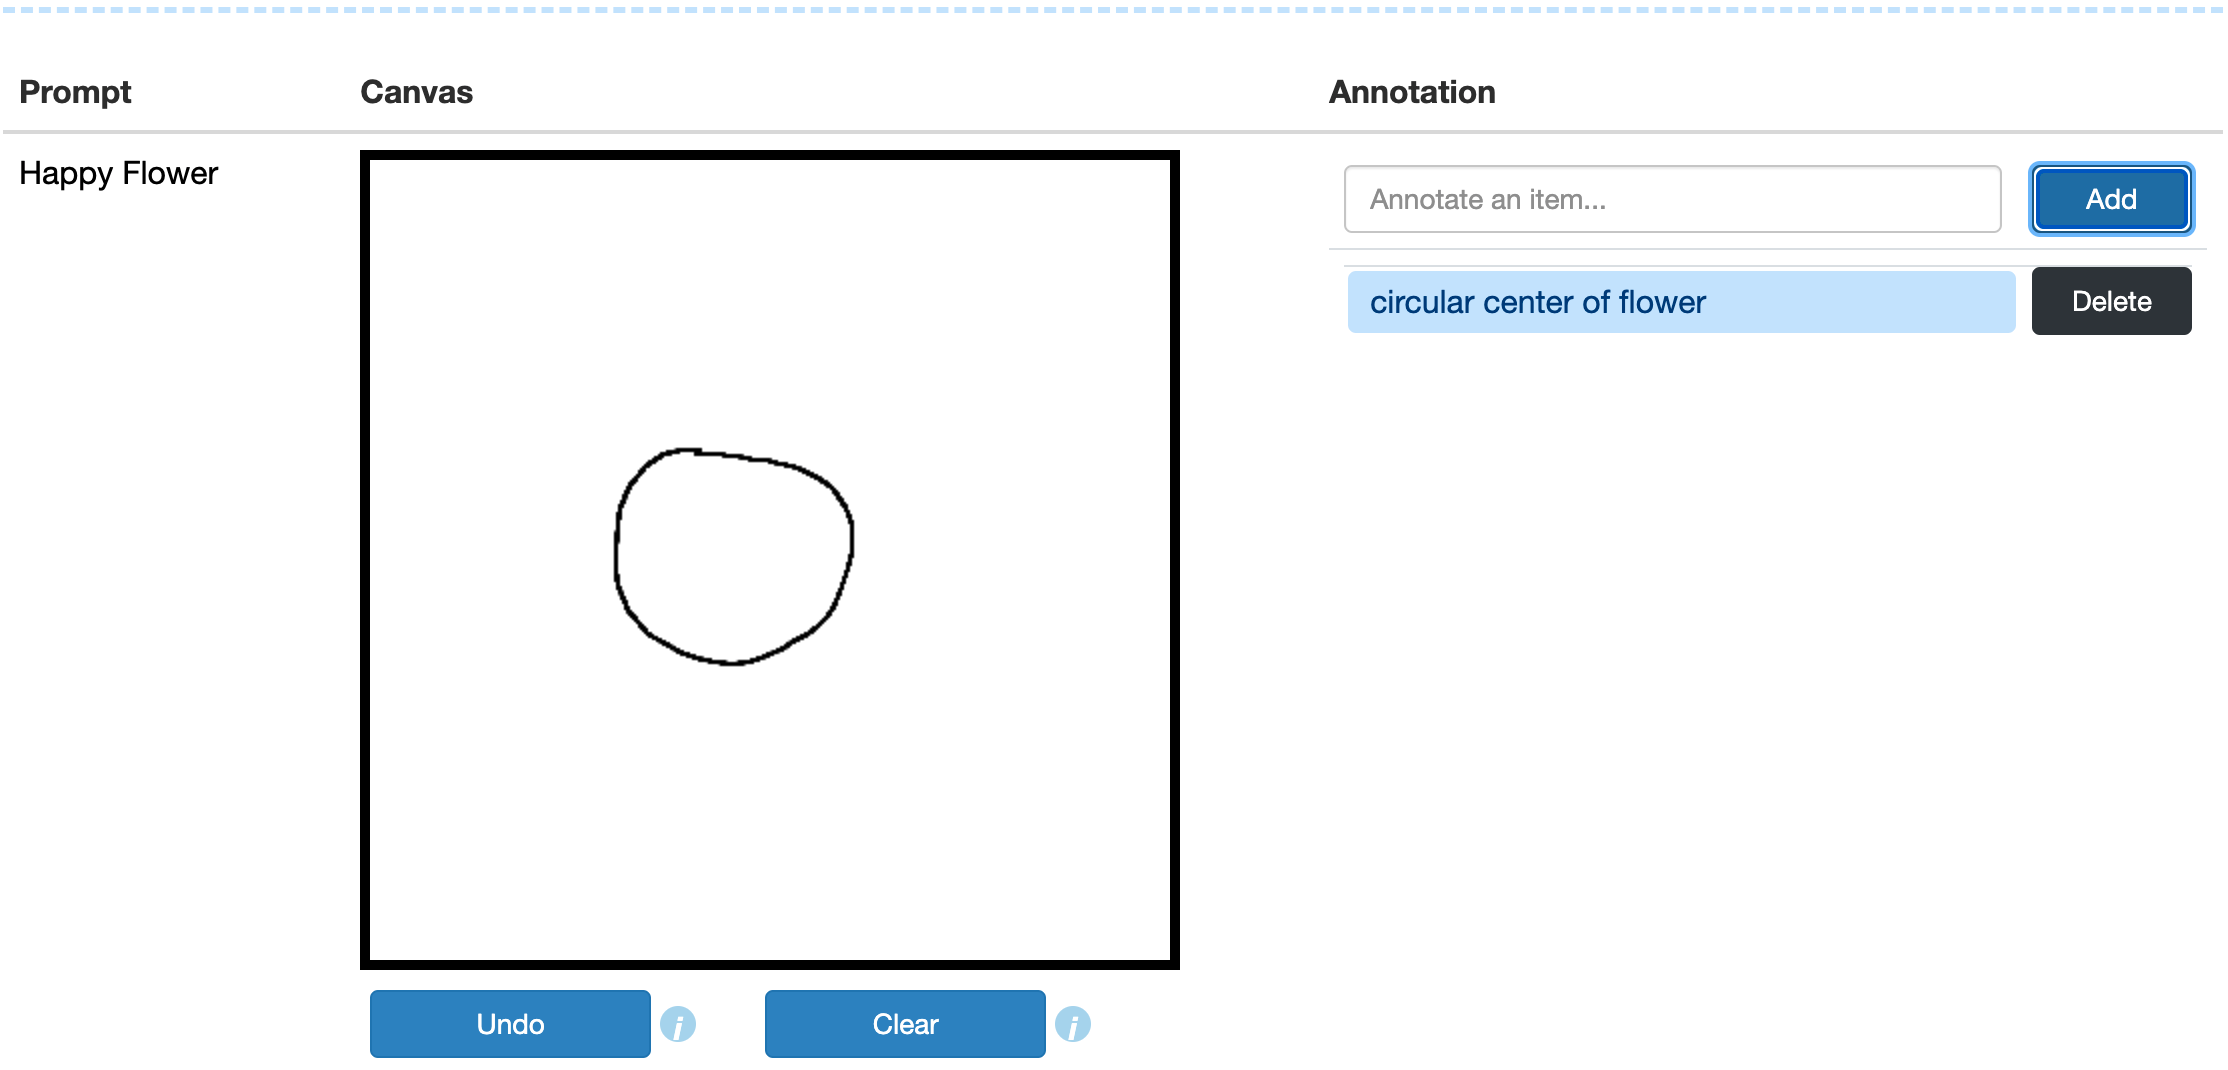
\includegraphics[width=.8\linewidth]{data_collection/v1_after_enter_text.png}  
    \caption{Main task interface after adding textual descriptions for the drawing in the given step.}
    \label{v1.main_task.1.c}
\end{subfigure}
\caption{The ``drawing-and-adding'' functionality in Version 1. Repeat the above process for each step in a sketch.}
\label{v1.main_task.1}
\end{figure*}

We illustrate a typical annotation process with version 1's interface in Figure \ref{v1.main_task.1}. 
The annotator starts with an empty canvas and empty table for textual descriptions, as shown in Figure \ref{v1.main_task.1.a}. For the annotator's convenience, we include a \textit{Undo} button and a \textit{Clear} button for erasing strokes and clearing entire canvas.  
Then, the annotator draws a step in the sketch, and they would need to enter into the \textit{Annotation} column and hit \textit{Add} to enter textual description into the annotation table. (Figure \ref{v1.main_task.1.b} and \ref{v1.main_task.1.c} show what the annotation table looks like before and after adding the texts for a given step.)
Repeat the drawing-and-adding process until the drawing is done. 

\begin{figure*}[!htb]
\begin{subfigure}{\textwidth}
    \centering
    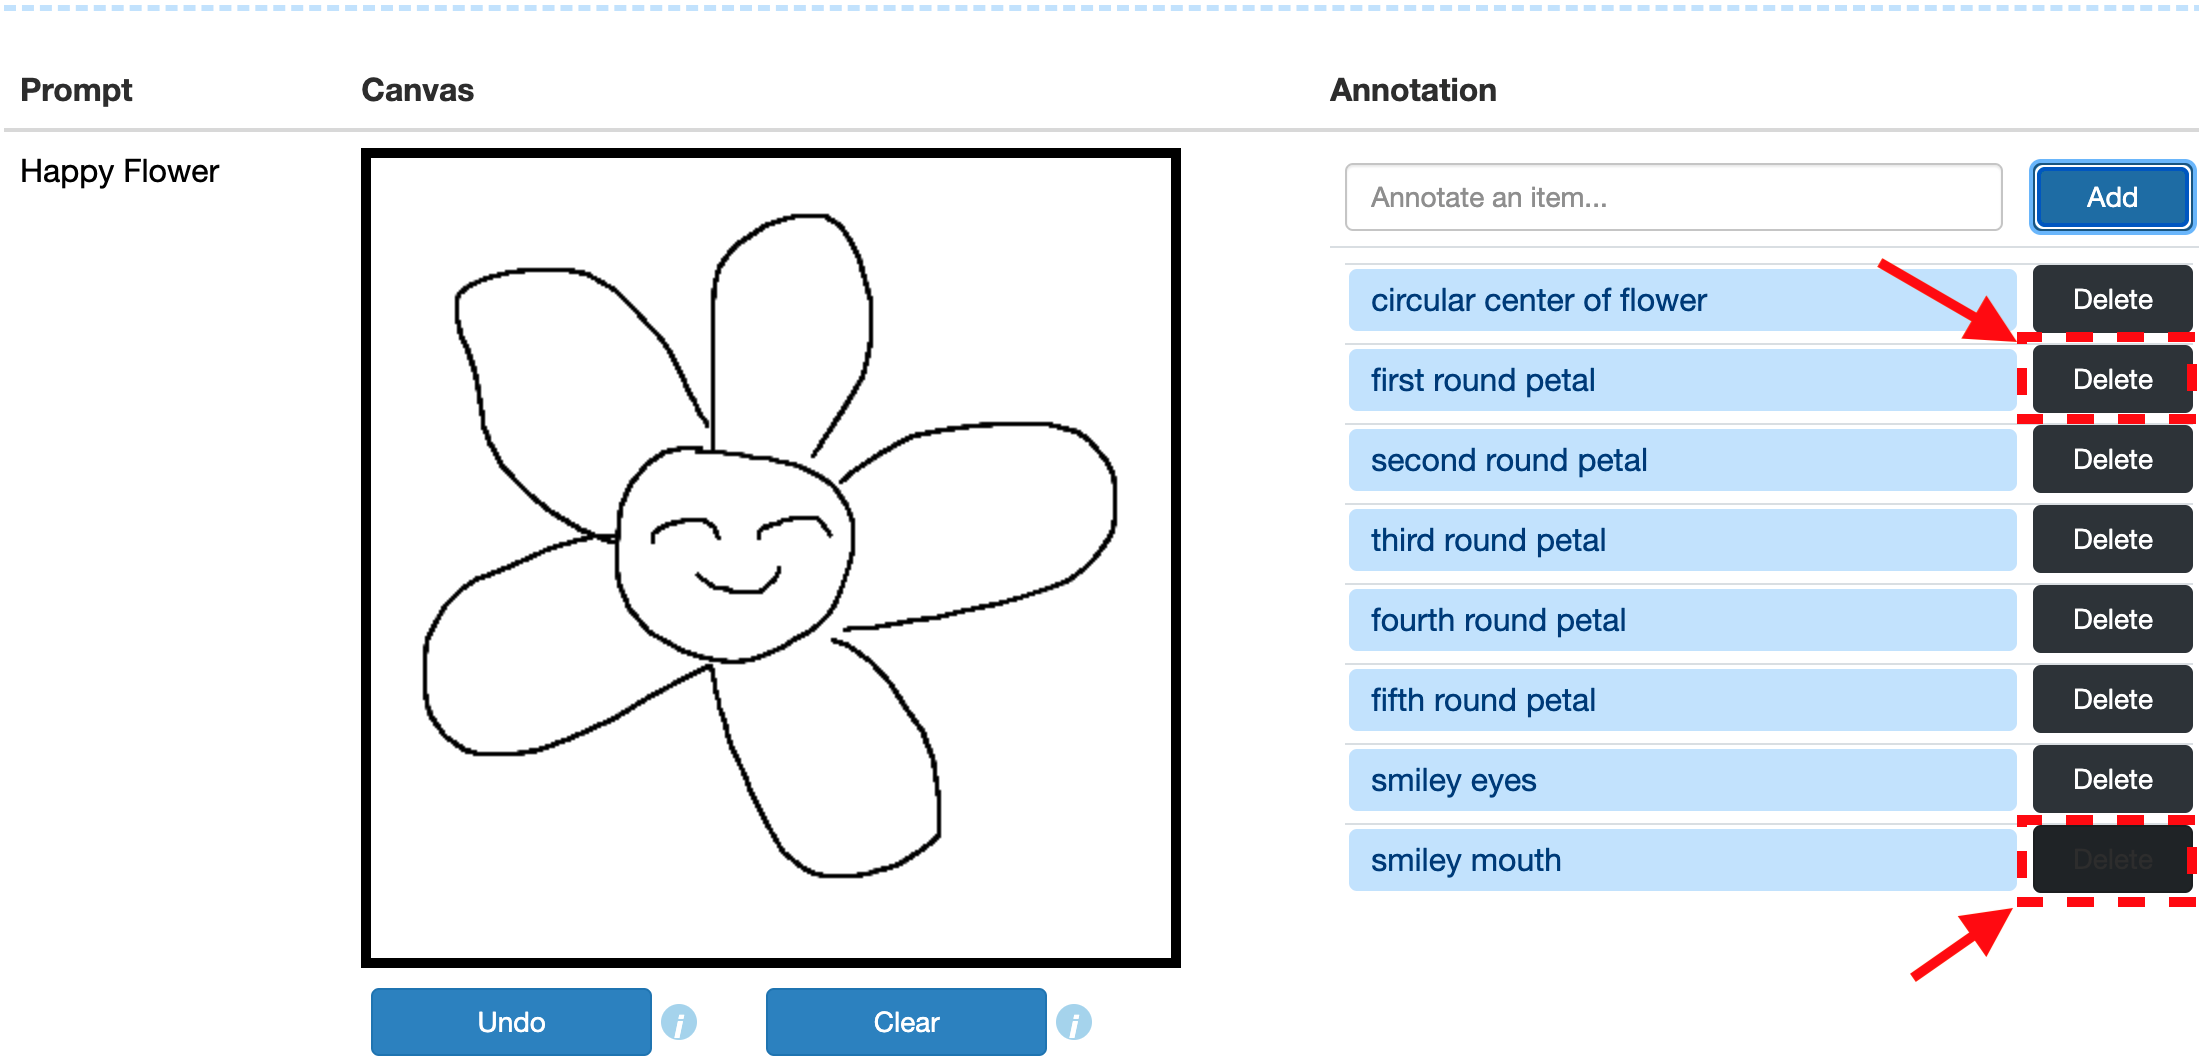
\includegraphics[width=.8\linewidth]{data_collection/v1_before_delete.png}  
    \caption{A complete annotation for the prompt \textit{Happy Flower}. Red arrows and boxes point to \textit{Delete} buttons that can be used to delete the steps associated with the textual annotaitons, if the annotator is not satisfied with the steps.}
    \label{v1.main_task.delete.a}
\end{subfigure}
\newline
\begin{subfigure}{\textwidth}
    \centering
    % include third image
    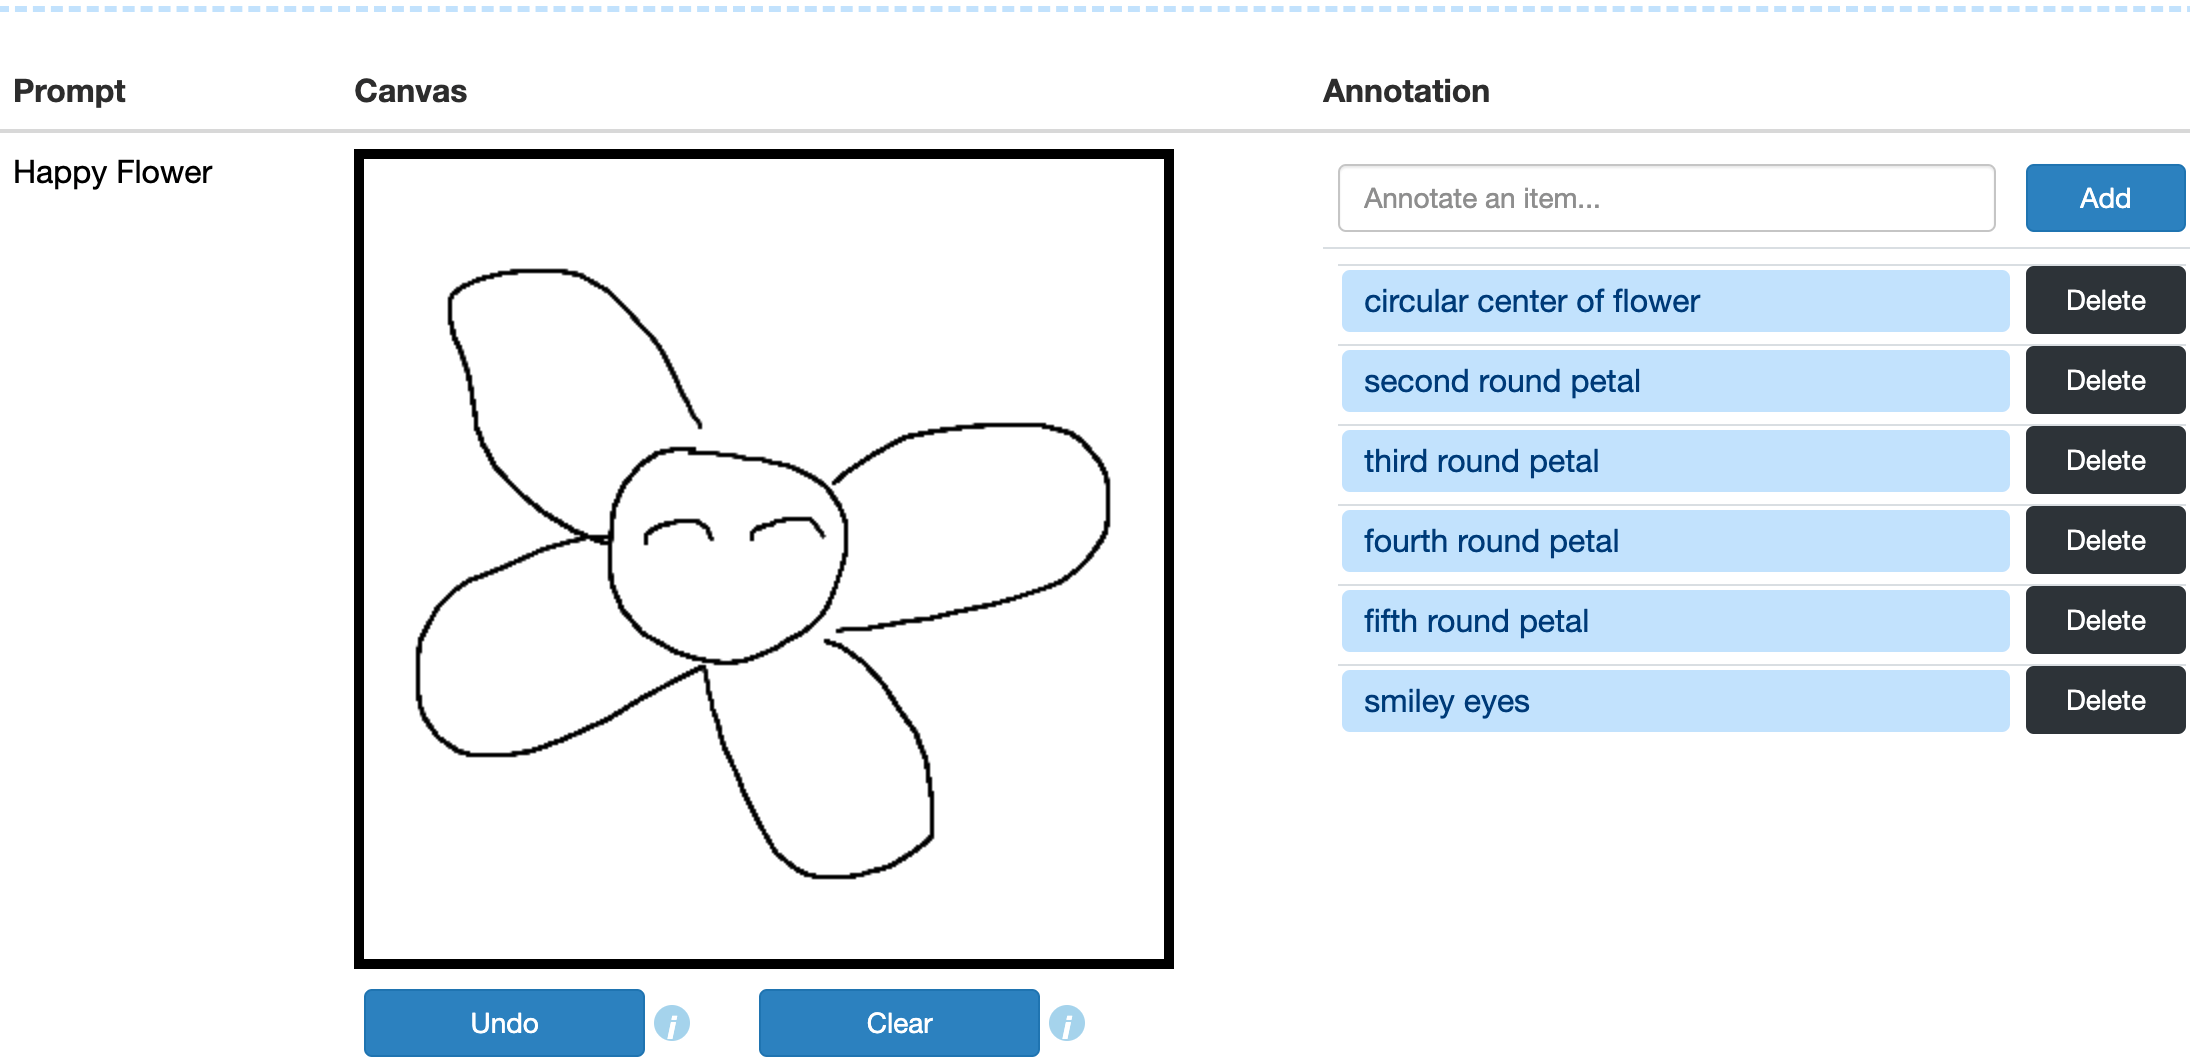
\includegraphics[width=.8\linewidth]{data_collection/v1_after_delete.png}  
    \caption{Main task interface after the two steps associated with \textit{first round petal} and \textit{smiley mouth}, respectively.}
    \label{v1.main_task.delete.b}
\end{subfigure}
\caption{Demonstrating the functionality of the \textit{Delete} button.}
\label{v1.main_task.delete}
\end{figure*}


If the annotator wants to remove an entire object in the drawing, they can use the \textit{Delete} button next to the texts to delete an entire object. An example is shown in Figure \ref{v1.main_task.delete}. \textit{Delete} an annotation together with its drawing on the board. Do not erase overlapping strokes. Constructing something like layers used in Photoshop, so that each step is its separate canvas layer. 
Adding annotations for each part in the drawing is done through a table. The design of using a table seeks to help annotators to keep track of which steps are annotated. Since in the requirement, we would specify how many steps are required in minimum for the annotation, so the table also helps to enforce DQ \ref{data_design_2} and \ref{data_design_3}. Enabling users to be able to delete each component is also demonstrative of these two DQ's. 



\subsubsection{Instruction and Requirement}
For the instructions, we mainly just illustrated the layout of the main task interface, as shown in Figure x3.
[Figure x3: including progress of previous instructions]
The first thing we spent time considering was how much motivation should we give about the task. Why are we conducting this survey? The second, more important, aspect to consider is what defines a single \textit{step} in the data that we collect. Should the annotator be asked to annotate for each stroke? However, this option is not only time-consuming but also fails to align with how a person would talk when, for example, teaching a child how to draw. Therefore, we decided that the annotator should annotate for each \textit{object} in the drawing. The ambiguity surrounding the word \textit{object} has been the biggest challenge in defining a clear set of requirements for the annotators. For example, when drawing for the prompt \textit{happy face}, one reasonable decomposition is annotating for 4 steps: face, eyes, mouth, and the face contour. However, for someone who draws very detailed eyes, they might want to annotate for the shape of the eye socket and the length of the eye lashes. It seems like there is a wide spectrum of allowed annotations depending on how one would approach drawing for the give prompt. Indeed, the great uncertainty that comes from individuality and personal styles of collecting drawings from turkers would eventually drive us to not collect drawings and simply annotate for sketches found in existing datasets.                    

A lot of effort went into defining what is the basic element of the annotation. We tried item, object, component. The goal of the model is to conditioned on previous steps to produce the next part. Figure 3x.a and 3x.b show some previous versions of the instructions. We eventually decided that  

There is even more effort that went into defining the requirements of the task. This is really the section that we want to use to enforce all the DQ's. The final set of instructions is displayed in Figure x4.
[Figure x4: final requirements]

Comparing examples in requirements format:

Methods to help understand the requirements. 
Specifying which examples demonstrate which requirements, add next to the questions which requirement the question is testing. 



\subsubsection{Qualification}

A qualification test is setup on AMT to train turkers to have better understanding of the task, and it is also used to select a group of turkers who can provide annotations that satisfy all the requirements. The full test is illustrated in Figure x5.

[Figure x5: final qualification test]

To come up with a set of questions that have good correspondence with the requirements, we went through several rounds of testing with students in the lab.  

The format of the qualification has also went through transformed, as shown in Figure x6. At first, we asked the annotators to select which steps of the annotations satisfy the requirements (Figure x6.a); in order to use repetition to ensure deep understanding of the requirements, we changed to asking a yes/no question for every step, as shown in Figure x6.b.  

[Figure x6]

\subsection{Deployment Results}

In order to determine how feasible the task is, we first deployed a version among lab members, and we obtained 55 drawings along with their annotations. All 55 drawings are shown in Figure v1.results.2. Some examples of step annotations are shown in Figure v1.results.3.  

[Figure v1.results.2: 55 drawings from lab deployment (see jupyter notebook oct\_28\_trial\_analysis)]
[Figure v1.results.3: 3 examples?]

To come up with a set of prompts to test for the first pilot, we want to come up with prompts in the forms of \textit{adjective}$\times$\textit{noun}. The list of adjectives includes: \textit{happy}, \textit{sad}, \textit{surprised},\textit{sleepy},\textit{lovestruck},\textit{evil}; the list of nouns includes: \textit{person}, \textit{kid}, \textit{cat}, \textit{bear}, \textit{dog}, \textit{sheep}, \textit{jellyfish}, \textit{cup of boba}, \textit{apple}, \textit{burger}, \textit{sun}, \textit{moon}, \textit{star}. We hope to test whether annotators can draw for abstract prompts like. Morever, we wish to see whether steps can be clearly annotated for these abstract prompts. It was also motivated by the fact that current AI-generated artwork like those produced by DALL-E often test its methods with abstract prompts, and the hope was that our collaborative agent can also respond to these prompts through interactive drawing.   

[Figure v1.results.4: drawings from the amt pilot]

What surprised us was the amount of time turkers spent on the task. Histograms of time each annotator spent on the task is illustrated in Figure v1.results.1. Statistics of the distributions are shown in Table v1.results.1. The discrepancy might be caused by the fact that lab members with their background in computer science have an implicit understandings of what kind of quality data are needed to train ML models.   

[Figure v1.results.1: a: oct 28 lab deployment. b: dec 28 amt deployment]
[Table v1.results.1: comparing the statistics of lab vs. amt deployment]

In violation of DQ \ref{data_design_1}. Drawing does not illustrate the prompt well. The quality of the drawings are greatly influenced by how well the annotator can understand the prompts. Drawing is by its nature very subjective, so when we were examining through the sketches that we collected, we were not able to understand in what ways some sketches convey the prompts. 
[Figure v1.results.4: some examples of sketches that cannot illustrate the prompt from our perspective]

In violation of DQ \ref{data_design_2} and \ref{data_design_3}. Another problem was that annotators often fail to describe every parts they drew in one step, or the descriptions miss some parts in the step, or the description does not align well with the drawings.   
[Figure v1.results.5: some examples of mis-aligned descriptions]